\documentclass{bioinfo}
\copyrightyear{2014}
\pubyear{2014}
\usepackage{amsmath}
\usepackage{afterpage}
\usepackage{algorithm}
\usepackage{float}
\usepackage{bbm}
\usepackage{subfig}
\usepackage{wrapfig}
\usepackage[font={small}]{caption}
\usepackage[skip=2pt,font=scriptsize]{caption}
%\usepackage{placeins}
\usepackage{algpseudocode}% http://ctan.org/pkg/algorithmicx
\usepackage{xr}
\externaldocument{supplementary_info}
\algnewcommand{\LineComment}[1]{\State \(\triangleright\) #1}

\newcommand{\RR}{I\!\!R} %real numbers
\DeclareMathOperator{\diag}{diag}
\begin{document}
\firstpage{1}

\title[RVD2]{RVD2: An ultra-sensitive variant detection model for low-depth heterogeneous next-generation sequencing data}
\author[He \textit{et~al}]{Yuting He\,$^{1}$, Patrick Flaherty\,$^{1}$\footnote{Corresponding Author: pjflaherty@wpi.edu}}
\address{$^{1}$Department of Biomedical Engineering, Worcester Polytechnic Institute, Worcester, MA, USA}

\history{Received on XXXXX; revised on XXXXX; accepted on XXXXX}

\editor{Associate Editor: XXXXXXX}

\maketitle

\begin{abstract}

\section{Motivation:}Next-generation sequencing technology is increasingly being used for clinical diagnostic tests. Unlike research cell lines, clinical samples are often genomically heterogeneous due to low sample purity or the presence of genetic subpopulations. Therefore, a variant calling algorithm for calling low-frequency polymorphisms in heterogeneous samples is needed.

\section{Results:}We present a novel variant calling algorithm that uses a hierarchical Bayesian model to estimate allele frequency and call variants in heterogeneous samples. We show that our algorithm improves upon current classifiers and has higher sensitivity and specificity over a wide range of median read depth and minor allele frequency. We apply our model and identify twelve mutations in the PAXP1 gene in a matched clinical breast ductal carcinoma tumor sample; two of which are loss-of-heterozygosity events.


\section{Availability:}
\href{http://genomics.wpi.edu/rvd2/}{http://genomics.wpi.edu/rvd2/}

\section{Contact:} \href{pjflaherty@wpi.edu}{pjflaherty@wpi.edu}
\end{abstract}

\section{Introduction}
\label{sec:intro}
Next-generation sequencing (NGS) technology has enabled the systematic interrogation of the genome for a fraction of the cost of traditional assays~\citep{Koboldt:2013kw}. Protocol and platform engineering improvements have enabled the generation of $1\times10^9$ bases of sequence data in 27 hours for approximately \$1000~\citep{Quail:2012hf}. As a result, NGS is increasingly being used as a general platform for research assays for methylation state~\citep{Laird:2010ab}, DNA mutations~\citep{Consortium:2013co}, copy number variation~\citep{Alkan:2009cr}, promoter occupancy~\citep{Ouyang:2009hc} and others~\citep{Rivera:2013ee}. NGS diagnostics are being translated to clinical applications including noninvasive fetal diagnostics~\citep{Kitzman:2012hea}, infectious disease diagnostics~\citep{Capobianchi:2012em}, cancer diagnostics~\citep{Navin:2010gu}, and human microbial analysis~\citep{Consortium:2013iz}.

Increasingly, NGS is being used to interrogate mutations in heterogeneous clinical samples. For example, NGS-based non-invasive fetal DNA testing uses maternal blood sample to sequence the minority fraction of cell-free fetal DNA~\citep{Fan:2008di}. Infectious diseases such as HIV and influenza may contain many genetically heterogeneous sub-populations~\citep{Flaherty:2011ja, Ghedin:2010ie}. DNA sequencing of individual regions of a solid tumor has revealed genetic heterogeneous within an individual sample~\citep{Navin:2010gu}. Importantly, accounting for technical errors can drastically improve performance~\citep{zagordi2010error}.

However, the primary statistical tools for calling variants from NGS data are optimized for homogeneous samples. Samtools and GATK use a naive Bayesian decision rule to call variants~\citep{li2011statistical, depristo2011framework}. GATK involves more sophisticate pre- and post-processing steps wherein the genotype prior is fixed and constant across all loci and the likelihood of an allele at a locus is a function of the phred score~\citep{McKenna:2010bv}.

Recently, some have developed algorithms to call low-frequency or rare variants in heterogeneous samples.~\citet{yau2010statistical} developed a Bayesian framework which can model the normal DNA contamination and intra-tumor heterogeneity by parameterizing the normal genotype cell proportion at each SNP. VarScan2 combines algorithmic heuristics to call genotypes in the tumor and normal sample pileup data and then applies a Fisher's exact test on the read count data to detect a significant difference in the genotype calls~\citep{Koboldt:2012cg}. Strelka uses a hierarchical Bayesian approach to model the joint distribution of the allele frequency in the tumor and normal samples at each locus~\citep{Saunders:2012fh}. With the joint distribution available, one is able to identify locations with dissimilar allele frequencies. muTect uses a Bayesian posterior probability in its decision rule to evaluate the likelihood of a mutation~\citep{Cibulskis:2013ta}. RVD uses a hierarchical Bayesian model to capture the error structure of the data and call variants~\citep{Flaherty:2011ja, cushing2013rvd}. That algorithm requires a very high read depth to estimate the sequencing error rate and call variants.


Several studies have compared the relative performance of these algorithms. \citet{spencer2013performance} demonstrated  that VarScan-somatic performed the best comparing with SAMtools, GATK and SPLINTER in detecting minor allele frequencies (MAFs) of 1\% to 8\%, with $ > $500× coverage required for optimal performance. However, \citet{spencer2013performance} also highlighted the fact that VarScan2 yielded more false positives at high read depth. \citet{Stead:2013fu} showed that VarScan-somatic outperformed Strelka and had performance on-par with muTect in detecting a 5\% MAF for read depths between 100 and 1000. %We test their performance on much lower MAF variants and across a wider range of coverage depths.

The remainder of this article is organized as follows. In the next section we describe the statistical model structure of our new algorithm, RVD2. Then, we derive a sampling algorithm for computing the posterior distribution over latent variables in the model and use those samples in a Bayesian posterior distribution hypothesis test to call variants. We compare the performance of RVD2 to several other variant calling algorithms for a range of read depths and minor allele fractions. Finally, we show that RVD2 is able to call variants on a heterogeneous clinical sample and identify two novel loss-of-heterozygosity events.

%%%%%%%%%%%%%%%%%%
% Model Structure
%%%%%%%%%%%%%%%%%%
\section{Model Structure}\label{sec:model_structure}

RVD2 uses a two-stage approach for detecting rare variants. First, it estimates the parameters of a hierarchical Bayesian model under two sequencing data sets: one from the sample of interest (case) and one from a known reference sample (control). Then, it tests for a significant difference between key model parameters in the case and control samples and returns called variant positions.

Figure~\ref{fig:graphical_model} shows a graphical representation of the RVD2 statistical model. In this graphical model framework a shaded node represents an observed random variable, an unshaded node represents an unobserved or latent random variable and a directed edge represents a functional dependency between the two connected nodes~\citep{jordan2004graphical}. A rounded box or ``plate" represents replication of the nodes within the plate. The graphical model framework connects graph theory and probability theory in a way that facilitates algorithmic methods for statistical inference.

\begin{figure}[!bpth]
\centering
\vspace{-10pt}
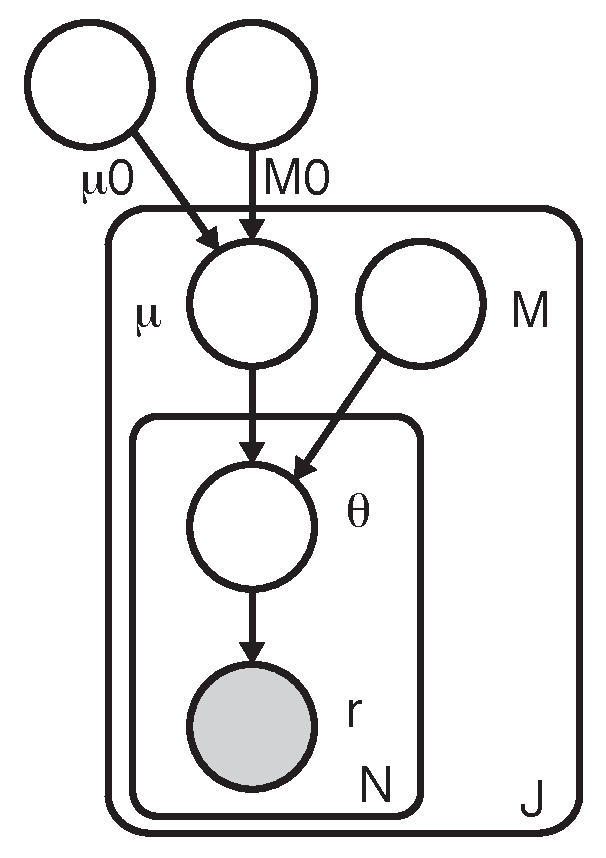
\includegraphics[width=33mm]{pdf_figs/RVD2_model.pdf}
\caption{RVD2 Graphical Model.}
\vspace{-20pt}
\label{fig:graphical_model}
\end{figure}

For a given sample, the observed data consists of two matrices $r \in \RR^{J \times N}$ and $n \in \RR^{J \times N}$, where $r_{ji}$ is the number of reads with a non-reference base at location $j$ in experimental replicate $i$ and $n_{ji}$ is the total number of reads at location $j$ in replicate $i$. $ J $ is the region of interest length and $ N $ is the number of technical replicates in the sample.\label{replicate definition} Technical replicates are used to establish experimental variability in next-generation sequencing procedure~\citep{robasky2013role}, though multiple replicates are not necessary for RVD2.
%~\citep{quackenbush2002microarray,robasky2013role}

The model generative process given hyperparameters $ \mu_0, M_0$ and $ M $is as follows:

\begin{enumerate}[noitemsep]
	\item For each location $j$:
	\begin{enumerate}[noitemsep]
		\item Draw an error rate $\mu_j \thicksim \text{Beta}(\mu_0, M_0)$
		\item For each replicate $i$:
		\begin{enumerate}
			\item Draw $\theta_{ji} \thicksim \text{Beta}(\mu_j, M_j)$
			\item Draw $r_{ji}|n_{ji} \thicksim \text{Binomial}(\theta_{ji}, n_{ji})$
		\end{enumerate}
	\end{enumerate}
\end{enumerate}

The generative process involves several hyperparameters: $\mu_0$, a global error rate; $M_0$, a global precision;  $ \mu_j $, a local error rate; and $M_j$, a local precision. The global error rate, $\mu_0$, estimates the expected error rate across all locations. The global precision, $M_0$, estimates the variation in the error rate  across locations. The local error rate, $ \mu_j $, estimates the exepected error rate across replicates at location $ j $. The local precision, $M_j$, estimates the variation in the error rate across replicates at location $j$.

RVD2 has three levels of sampling. First, a global error rate and global precision are chosen once for the entire data set. Then, at each location, a local precision is chosen and a local error rate is sampled from a Beta distribution. Finally, the error rate for replicate $i$ at location $j$ is drawn from a Beta distribution and the number of non-reference reads is drawn from a binomial.

RVD2 hierarchically partitions sources of variation in the data. The distribution $r_{ji} | n_{ji} \thicksim \text{Binomial}(\theta_{ji}, n_{ji})$ models the variation due to sampling the pool of DNA molecules on the sequencer. The distribution $\theta_{ji} \thicksim \text{Beta}(\mu_j, M_j)$ models the variation due to experimental reproducibility. The variation in error rate due to sequence context is modeled by $\mu_j \thicksim \text{Beta}(\mu_0, M_0)$. Importantly, increasing the read depth $n_{ji}$ only reduces the sampling error, but does nothing to reduce experimental variation or variation due to sequence context.


The joint distribution over the latent and observed variables for data at location $j$ in replicate $i$ given the parameters can be factorized as
\begin{multline}\label{eqn:jointpdf}
p \left( r_{ji}, \theta_{ji}, \mu_j | n_{ji}; \mu_0, M_0, M_j \right) \\ = p \left( r_{ji} | \theta_{ji}, n_{ji} \right) p\left( \theta_{ji} | \mu_j; M_j \right) p\left( \mu_j; \mu_0, M_0 \right),
\end{multline}

\begin{align}\nonumber
  p\left( r_{ji} | \theta_{ji}, n_{ji} \right) &= \frac{ \Gamma(n_{ji}+1) } { \Gamma(r_{ji}+1) \Gamma( n_{ji} - r_{ji} + 1 ) } \cdot \theta_{ji}^{r_{ji}} (1 - \theta_{ji})^{n_{ji} - r_{ji}}, \nonumber \\
 %
  p\left( \theta_{ji} | \mu_j; M_j \right) &= \dfrac{ \theta_{ji}^{M_j\mu_j -1} (1 - \theta_{ji})^{M_j ( 1 - \mu_j) - 1}}{\textbf{B}(M_j \mu_j, M_j (1-\mu_j))}, \nonumber \\
 %  
  p\left( \mu_j; \mu_0, M_0 \right)  &= \dfrac{\mu_j^{M_0\mu_0 -1} (1 - \mu_j)^{M_0 ( 1 - \mu_0) - 1}}{\textbf{B}(M_0 \mu_0,M_0 (1-\mu_0) )}, \nonumber 
\end{align}
where \textbf{B}(x,y) denotes the beta function.
%Integrating over the latent variables $\theta_{ji}$ and $\mu_j$ yields the marginal distribution of the data,
%\begin{multline}
%p \left( r_{ji} | n_{ji} ; \mu_0, M_0, M_j \right) = \int_{\mu_j} \int_{\theta_{ji}}  p \left( r_{ji} | \theta_{ji}, n_{ji} \right) \\ p\left( \theta_{ji} | \mu_j; M_j \right) p\left( \mu_j; \mu_0, M_0 \right) d\theta_{ji} d\mu_j.
%\end{multline}

The log-likelihood of the data set is
\begin{multline}
\log p \left( r | n ; \mu_0, M_0, M \right) = \sum_{j=1}^J \sum_{i=1}^N \log \int_{\mu_j} \int_{\theta_{ji}}  p \left( r_{ji} | \theta_{ji}, n_{ji} \right) \\ p\left( \theta_{ji} | \mu_j; M_j \right) p\left( \mu_j; \mu_0, M_0 \right) d\theta_{ji} d\mu_j.
\end{multline}

\label{Improvement of RVD2}
RVD2 improves on RVD in three ways. First, RVD2 has a $ \text{Beta}(\mu_0, M_0) $ prior on local error rate $ \mu_j $, which captures the global across-position error rate. The prior distribution allows $ \mu_j $ to borrow information from adjacent positions and allows RVD2 to handle low read depths. Second, RVD2 handles multiple replicates in case samples. Third, RVD2 has a more accurate Bayesian hypothesis testing method compared to a frequentist normal z-test in RVD. We show a performance comparison between RVD and RVD2 in Section~\ref{sec:comparison}.

%%%%%%%%%%%%%%%%%%
% Inference & Hypothesis Testing
%%%%%%%%%%%%%%%%%%
\section{Inference and Hypothesis Testing}

The primary object of inference in this model is the joint posterior distribution function over the latent variables,
\begin{equation}
	p(\mu, \theta | r, n; \phi)  = \frac{ p(\mu, \theta, r | n; \phi) } {p ( r | n; \phi)},
\end{equation}
where the parameters are $\phi \triangleq \{\mu_0, M_0, M\}$.

The Beta distribution over $\mu_j$ is conjugate to the Binomial distribution over $\theta_{ji}$, so we can write the posterior distribution as a Beta distribution. However, there is not a closed form for the product of a Beta distribution with another Beta distribution, so exact inference is intractable.

Instead, we have developed a Metropolis-within-Gibbs  approximate inference algorithm shown in Algorithm~\ref{alg:metro_gibbs}. First, the hyperparameters are initialized using method-of-moments (MoM). Given those hyperparameter estimates, we sample from the marginal posterior distribution for $\mu_j$ given its Markov blanket using a Metropolis-Hasting rejection sampling rule. Finally, we sample from the marginal posterior distribution for $\theta_{ji}$ given its Markov blanket. Samples from $\theta_{ji}$ can be drawn from the posterior distribution directly  because the prior and likelihood form a conjugate pair. This sampling procedure is repeated until the chain converges to a stationary distribution and then we draw samples from the posterior distribution over latent variables.

\begin{algorithm}[ht]
  \caption{Metropolis-within-Gibbs Algorithm}
  \label{alg:metro_gibbs}
  \begin{algorithmic}[1]

  \State Initialize $\theta$, $\mu$, $M$, $\mu_0$, $M_0$

  \Repeat

    \For {each location j}

    \State Draw T samples from $p \left( \mu_j |\theta_{ij},\mu_0,M_0\right)$ using M--H 
   % \Comment{Sample $\mu_j$}

    \State Set $\mu_j$ to the sample median for the T samples

      \For {each replicate i}

	\State Sample from $p \left( \theta_{ij} |r_{ij},n_{ij},\mu_j,M \right)$
	%\Comment{Sample $\theta_{ji}$}
	
      \EndFor

    \EndFor

  \Until {sample size sufficient}

  \end{algorithmic}
\end{algorithm}


%%%%%%%%%%%%%
% Initialization
%%%%%%%%%%%%%
\vspace{-20pt}
\subsection{Initialization}
The initial values for the model parameters and latent variables are obtained by a method-of-moments (MoM) procedure. MoM works by setting the population moment equal to the sample moment. A system of equations is formed such that the number of moment equations is equal to the number of unknown parameters and the equations are solved simultaneously to give the parameter estimates. We simply start with the data matrices $r$ and $n$ and work up the hierarchy of the graphical model solving for the parameters of each conditional distribution in turn.

We present the initial parameter estimates here and provide the derivations in Supplementary Information. The MoM estimate for replicate-level parameters are
$\hat{\theta}_{ji} = \frac{r_{ji}} {n_{ji}}$.
The estimates for the position-level parameters are
$\hat{\mu}_j = \frac{1}{N} \sum_{i=1}^N \hat{\theta}_{ji}$
and
$\hat{M_j} = \frac{ \hat{\mu}_j (1 - \hat{\mu}_j ) } { \frac{1}{N} \sum_{i=1}^N \hat{\theta}_{ji}^2 } -1$.
The estimates for the genome-level parameters are
$\hat{\mu}_0 = \frac{1}{J} \sum_{j=1}^J \hat{\mu}_j$
and
$\hat{M}_0 = \frac{ \hat{\mu}_0 (1 - \hat{\mu}_0 ) } {\frac{1}{J} \sum_{j=1}^J \hat{\mu}_j^2 } -1$.
%While MoM is known to have the potential to return estimates outside the true parameter bounds, we have not encountered such behavior in this application.

%%%%%%%%%%%%%%%%%%
% Sampling theta
%%%%%%%%%%%%%%%%%%
\subsection{Sampling from $p \left( \theta_{ij} |r_{ij},n_{ij},\mu_j,M \right)$}

Samples from the posterior distribution
$p(\theta_{ji} | r_{ji}, n_{ji}, \mu_j, M_j)$
are drawn analytically because of the Bayesian conjugacy between the prior
$p(\theta_{ji} | \mu_j, M_j) \thicksim \text{Beta}(\mu_j, M_j)$
and the likelihood
$p(r_{ji} | n_{ji}, \theta_{ji}) \thicksim \text{Binomial}(\theta_{ji}, n_{ji})$.
The posterior distribution is
\begin{flalign}
& p(\theta_{ji} | r_{ji}, n_{ji}, \mu_j, M_j)& \nonumber \\
& \thicksim\text {Beta}\left( r_{ji} + M_j \mu_j , n_{ji}- r_{ji} + M_j (1-\mu_j)\right).&
\end{flalign}

%%%%%%%%%%%%%%%%%%
% Sampling mu
%%%%%%%%%%%%%%%%%%
\subsection{Sampling from $p \left( \mu_j |\theta_{ji},M_j,\mu_0,M_0\right)$}
The posterior distribution over $\mu_j$ given its Markov blanket is
\begin{equation}
	p( \mu_j | \theta_{ji}, M_j, \mu_0, M_0 ) \propto p(\mu_j | \mu_0, M_0) p(\theta_{ji} | \mu_j, M_j).
\end{equation}

Since the prior, $p(\mu_j | \mu_0, M_0)$, is not conjugate to the likelihood, $p(\theta_{ji} | \mu_j, M_j)$, we cannot write an analytical form for the posterior distribution. Instead, we sample from the posterior distribution using the Metropolis-Hastings algorithm.

A candidate sample is generated from the symmetric proposal distribution $Q(\mu_j^* | \mu_j^{(p)}) \thicksim \mathcal{N}(\mu_j^{(p)}, \sigma_j^2)$, where $\mu_j^{(p)}$ is the $p$th from the posterior distribution. The acceptance probability is then
\begin{equation}
	a = \frac{ p(\mu_j^* | \mu_0, M_0) p(\theta^{(p+1)}_{ji} | \mu_j^*, M_j) } {p(\mu_j^{(p)} | \mu_0, M_0) p(\theta^{(p+1)}_{ji} | \mu_j^{(p)}, M_j)}
\end{equation}

We fixed the proposal distribution variance for all the Metropolis-Hastings steps within a Gibbs iteration to $\sigma_j = 0.1 \cdot \hat{\mu}_j\cdot (1-\hat{\mu}_j)$ if $\hat{\mu}_j \in (10^{-3},1-10^{-3})$ and $\sigma_j = 10^{-4}$ otherwise, where $\hat{\mu}_j$ is the MoM estimator of $\mu_j$. Though it is not theoretically necessary, we have found that the algorithm performance improves when we take the median of five or more M-H samples as a single Gibbs step for each position.


We resample from the proposal if the sample is outside of the support of the posterior distribution. We typically discard 20\% of the sample for burn-in and thin the chain by a factor of 2 to reduce autocorrelation among samples. Since, each position $j$ is exchangeable given the global hyperparameters, $\mu_0$ and $M_0$, this sampling step can be distributed across up to $J$ processors.

%%%%%%%%%%%%%%%%%%
% Posterior Distribution Test
%%%%%%%%%%%%%%%%%%
\subsection{Posterior Distribution Test}\label{sec:hypothesis_test}
\subsubsection*{Posterior Difference Test.}
Metropolis-within-Gibbs provides samples from the posterior distribution of $\mu_j$ given the case or control data. For notational simplicity, we define the random variables associated with these two distributions $\mu_j^{\text{case}}$ and $\mu_j^{\text{control}}$ and the associated samples as $\tilde{\mu}_j^{\text{case}}$ and $\tilde{\mu}_j^{\text{control}}$.

A variant is called if $\mu_j^{\text{case}} > \mu_j^{\text{control}}$ with high confidence,
\begin{equation}\label{eqn:bayes_test}
	\Pr( \mu_j^{\text{case}} - \mu_j^{\text{control}}  > \tau ) \approx \frac{1}{N_{\text{MH}}} \sum_{k=1}^{N_{\text{MH}}} \mathbbm{1}_{\tilde{\mu}_{jk}^{\text{case}} - \tilde{\mu}_{jk}^{\text{control}} > \tau } > 1-\alpha,
\end{equation}
where $\tau$ is a detection threshold and $1-\alpha$ is a confidence level. We draw a sample from the posterior distribution $\tilde{\mu}_j^{\Delta} \triangleq \tilde{\mu}_j^{\text{case}} - \tilde{\mu}_j^{\text{control}}$ by simple random sampling with replacement from $\tilde{\mu}_j^{\text{case}}$ and $\tilde{\mu}_j^{\text{control}}$.

The threshold, $\tau$, may be set to zero or optimized for a given median depth and desired MAF detection limit. The optimal $\tau$ maximizes the Matthews Correlation Coefficient (MCC),
\begin{equation}
	\tau^* = \arg\max_\tau \left\{ \text{MCC}(\tau)\right\}.
\end{equation}

While we are able to compute the optimal $\tau$ threshold for a test data set, in general we would not have access to $\tau^*$. With sufficient training data, one would be able to develop a lookup table or calibration curve to set $\tau$ based on read depth and MAF level of interest. Absent this information we set $\tau = 0$.

\subsubsection*{Posterior Somatic Test.}

We use a two-sided posterior difference test with control and case paired samples to identify somatic mutations. We consider scenarios when the case(tumor) error rate is lower than the control(germline) error rate (e.g. loss-of-heterozygosity) as well as scenarios when the case(tumor) error rate is higher than the control(germline) error rate (e.g. homozygous somatic mutation). The two hypothesis tests are then $\Pr( \mu_j^{\text{case}} - \mu_j^{\text{control}} > \tau ) > 1-\alpha$ and $\Pr( \mu_j^{\text{case}} - \mu_j^{\text{control}} < \tau ) > 1-\alpha$. We typically set the threshold $ \tau $ to zero.

\subsubsection*{Posterior Germline Test.}

We use a one-sided posterior distribution test with a single control sample to identify germline mutations. We call a germline mutation if $ \mu_j^{control} \geq \tau$ with high confidence,

\begin{equation}\label{eqn:germ_test}
	\Pr(\mu_j^{\text{control}}  \geq \tau ) \approx \frac{1}{N_{\text{MH}}} \sum_{k=1}^{N_{\text{MH}}} \mathbbm{1}_{\tilde{\mu}_{jk}^{\text{control}} \geq \tau } > 1-\alpha.
\end{equation}

%%%%%%%%%%%%%%%%%%
% Chi^2 Test
%%%%%%%%%%%%%%%%%%
\subsection{$\chi^2$ test for non-uniform base distribution}

An abundance of non-reference bases at a position called by the posterior density test may be due to a true mutation or due to a random sequencing error; we would like to differentiate these two scenarios. We assume non-reference read counts caused by a non-biological mechanism results in a uniform distribution over three non-reference bases. In contrast, the distribution of counts among three non-reference bases caused by biological mutation would not be uniform.

We use a $\chi^2$ goodness-of-fit test on a multinomial distribution over the non-reference bases to distinguish these two possible scenarios. The null hypothesis is $H_0: p = (p_1, p_2, p_3)$ where $p_1=p_2=p_3=1/3$. Cressie and Read (1984) identified a power-divergence family of statistics, indexed by $\lambda$, that includes as special cases Pearson's $\chi^2 (\lambda = 1)$ statistic, the log likelihood ratio statistic $(\lambda = 0)$, the Freeman-Tukey statistic $(\lambda = -1/2)$, and the Neyman modified statistic $X^2 (\lambda = -2)$. The test statistic is

\begin{equation}
 2nI^\lambda = \frac{2}{\lambda(\lambda+1)}\sum_{k=1}^3 r_{ji}^{(k)} \left[\left(\frac{r_{ji}^{(k)}}{E_{ji}^{(k)}}\right)^\lambda-1\right];\lambda \in R,
\end{equation}
where $r_{ji}^{(k)}$ is the observed frequency for non-reference base $k$ at position $j$ in replicate $i$ and $E_{ji}^{(k)}$ is the corresponding expected frequency under the null hypothesis. \citet{cressie1984multinomial} recommended $\lambda = 2/3$ when no knowledge of the alternative distribution is available and we choose that value.

We control for multiple hypothesis testing in two ways. We use Fisher's combined probability test \citep{fisher1970statistical} to combine the p-values for $N$ replicates into a single p-value at position $j$,

\begin{equation}\label{eqn:fisher_combined}
	X_j^2 = -2 \sum_{i=1}^N \ln(p_{ji}).
\end{equation}

Equation~\eqref{eqn:fisher_combined} gives a test statistic that follows a $\chi^2$ distribution with $2N$ degrees of freedom when the null hypothesis is true. If the sample average depth is higher than 500, we use the Benjamini-Hochberg method to control the family-wise error rate (FWER) over positions that have been called by the posterior distribution test \citep{benjamini1995controlling, efron2010large}. The average depth threshold is set because Benjamini-Hochberg method is a highly conservative method and will reject many true calls when the read depth is not high enough.

%%%%%%%%%%%%%%%%%%
% Data Sets
%%%%%%%%%%%%%%%%%%
\section{Data Sets}

We used two independent data sets to evaluate the performance of RVD2 and compare it with other variant calling algorithms. The synthetic DNA sequence data provides true positive and true negative positions as well as define minor allele fractions. The HCC1187 data is used to test the performance on a sequenced cancer genome with less than 100\% tumor purity.

\subsection{Synthetic DNA Sequence Data}

\subsubsection*{Experimental Methods.}
Two 400bp DNA sequences (including linkers) that are identical except at 14 loci with variant bases were synthesized and clonally isolated.
The samples with the mutations are taken as the case sample and the sample without the mutations is taken as the control. 
Aliquots of the case and control DNA were mixed at defined fractions to yield defined minor allele fractions (MAFs) of 0.1\%, 0.3\%, 1\%, 10\%, and 100\%. 
Paired-end sequencing was performed on an Illumina GAIIx sequencer (Illumina SCS 2.8) with real-time image analysis and base calling (Illumina RTA 2.8). 
Eland II (from Illumina pipeline version 1.6) was used with the default parameters to perform sequence alignment to the 300-bp synthetic DNA construct.
More details of the experimental protocol are available from the original publication~\citep{Flaherty:2011ja}.
As shown in Supplementary Table S1, each sample has approximately 1,000,000 35bp paired end reads.

\subsubsection*{Pre-processing Methods.}
The reads were aligned with Eland as described previously. We then ran samtools mpileup with the -C50 option to filter for high mapping quality reads. To simulate lower coverage data while retaining the error structure of real NGS data, BAM files for the synthetic DNA data were downsampled $10\times$, $100\times$, $1,000\times$, and $10,000\times$ using Picard v1.96. The final data set contains read pairs for three replicates of each case and pairs of reads three replicates for the control sample giving $N=6$ replicates for the control and each MAF level.

\subsection{HCC1187 Sequence Data}
\subsubsection*{Experimental Methods.}
The HCC1187 dataset is a well-recognized baseline dataset from Illumina for evaluating sequence analysis algorithms~\citep{newman2013relative,howarth2011large,howarth2007array}. The HCC1187 cell line was derived from  epithelial cells from primary breast tissue from a 41 y/o adult with TNM stage IIA primary ductal carcinoma. The estimated tumor purity was reported to be 0.8. Matched normal cells were derived from lymphoblastoid cells from peripheral blood. Sequencing libraries were prepared according to the protocol described in the original technical report~\citep{hcc1187techreport}.
\subsubsection*{Pre-processing Methods.}
 The raw FASTQ read files were aligned to hg19 using the Isaac aligner to generate BAM files~\citep{raczy2013isaac}. The aligned data had an average read depth of 40x for the normal sample and 90x for the tumor sample with about 96\% coverage with 10 or more reads. We used samtools mpileup to generate pileup files using hg19 as reference sequence~\citep{Navin:2010gu}.
%Not sure the author is correct
% HCC1187BL origin: http://www.atcc.org/products/all/CRL-2323.aspx


\section{Results}

We tested RVD2 using synthetic DNA and data from a primary ductal carcinoma sample. The inference algorithm parameters were set to yield $4,000$ Gibbs samples with a 20\% burn-in and $2\times$ thinning rate for a final total of $1,600$ samples. We drew $1,000$ samples from $ \tilde{\mu}^{\Delta} =  \tilde{\mu}_j^{\text{case}} - \tilde{\mu}_j^{\text{control}}$ to estimate the posterior probability of a variant.

We performed the posterior difference test to identify mutations in the haploid synthetic data. We set the threshold $ \tau =0 $ and the size of the test $ \alpha = 0.05$.

For the HCC1187 data set, we identified both somatic and germline mutations. In the posterior somatic test, we set the threshold $ \tau =0 $ and the size of the test $ \alpha = 0.05$. In the posterior germline test, We set  the threshold $ \tau =0.05 $ considering the low average coverage (40$\times$). The size of the test is set at $ \alpha = 0.15$. We performed the $\chi^2$ non-uniformity test after the posterior density tests.

\subsection{Performance by read depth}\label{sec:read_depth}

\begin{figure}[htbp]
\centering
\vspace{-15pt}
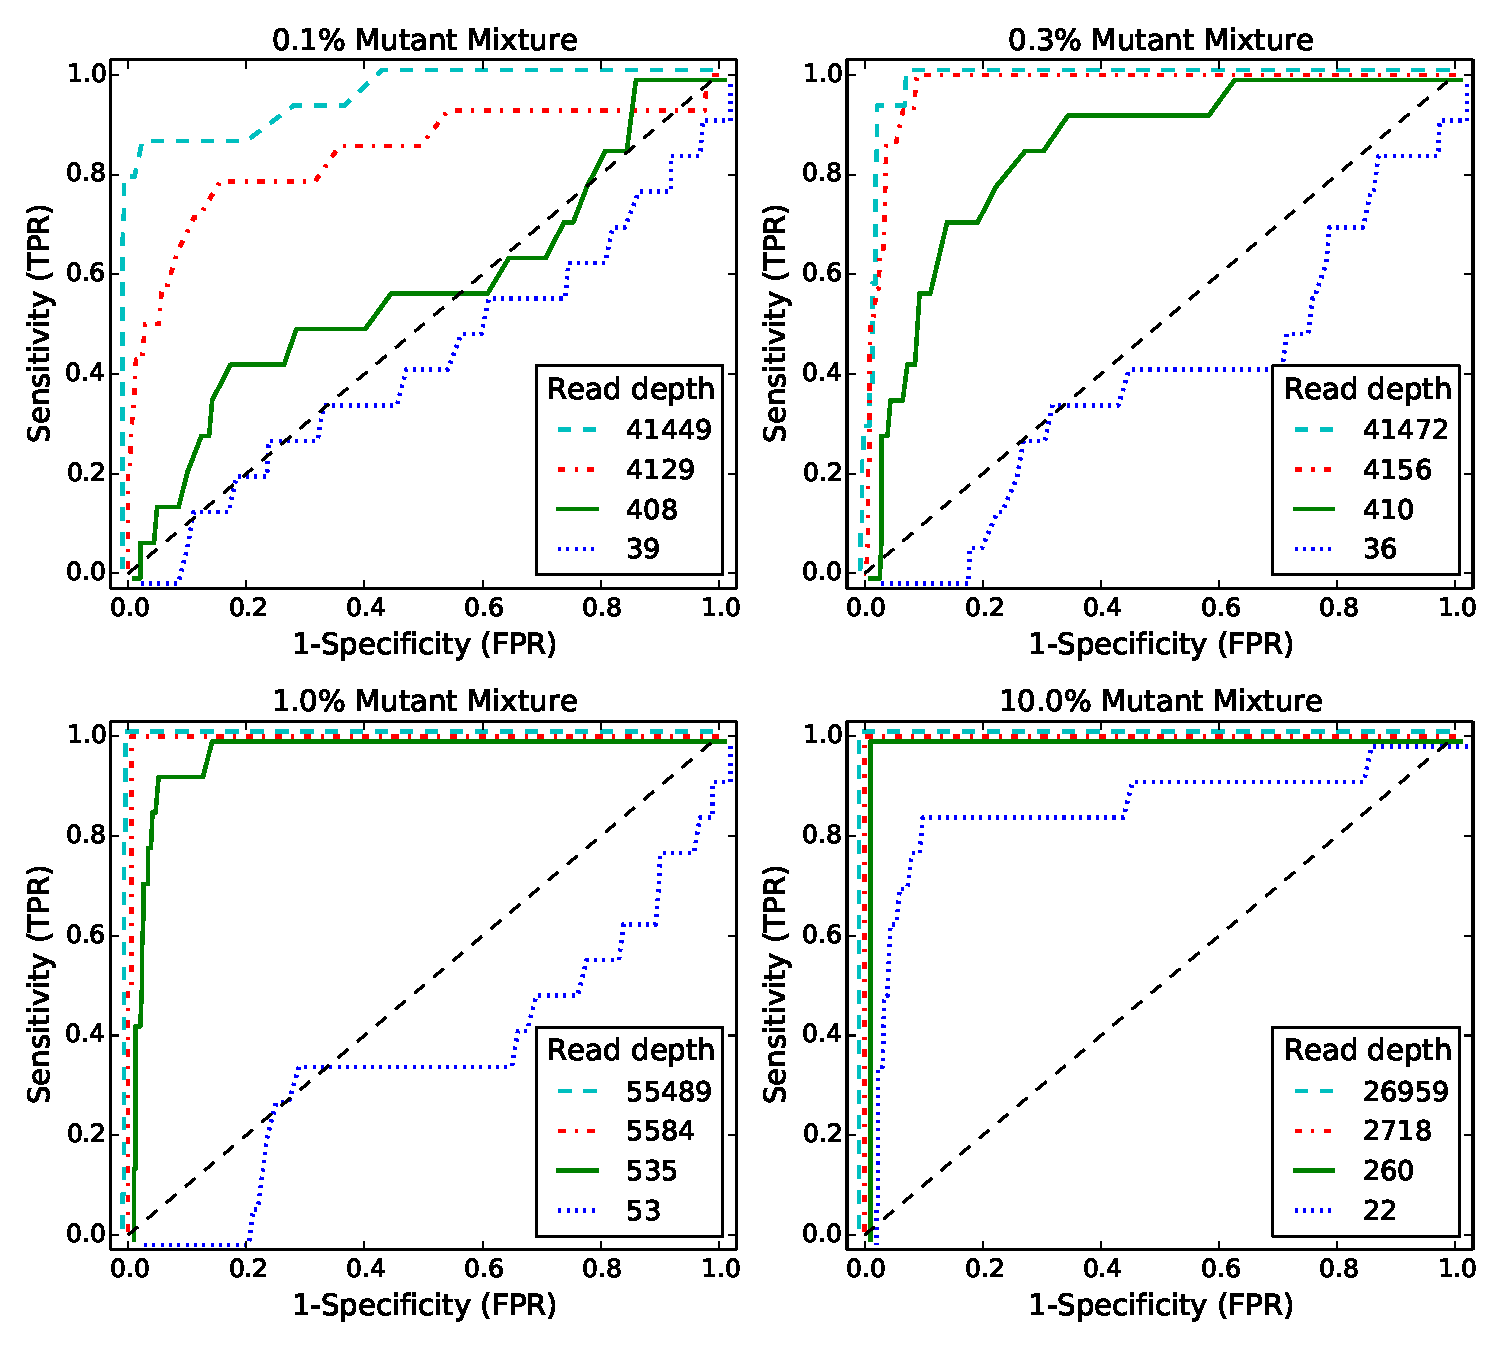
\includegraphics[width=0.45\textwidth]{pdf_figs/ROC_without_chi2.pdf}
\caption{ROC curve varying read depth showing detection performance. }
\vspace{-15pt}
\label{fig:ROC}
\end{figure}
We generated receiver-operating characteristic curves (ROCs) for a range of median read depth and a range of minor allele frequencies (MAFs). 
For these ROC curves, we used the posterior density test without the $\chi^2$ test to evaluate the performance of posterior density test individually. 
Figure~\ref{fig:ROC} shows ROC curves generated by varying the threshold $\tau$ with a fixed $\alpha=0.05$. 
Figure~\ref{fig:ROC}A shows ROC curves for a true 0.1\% MAF for a range of median coverage depths. 
At the lowest depth the sensitivity and specificity is no better than random. 
However, we would not expect to be able to call a 1 in 1000 variant base with a coverage of only 43. 
The performance improves monotonically with read depth. 
Figures~\ref{fig:ROC}B-C show a similar relationship between coverage depth and accuracy for higher MAFs.
% from folder '2013-11-24_six_replicates_Compute_ROC_Synthetic_Qsd_0_1'


\subsection{Empirical performance compared with other algorithms}\label{sec:comparison}

We compare the empirical performance of RVD2 to other variant calling algorithms using the synthetic DNA data set by the false discovery rate and sensitivity/specificity. 
Among these algorithms, Samtools and GATK are optimized for homogeneous samples, while RVD, VarScan2-somatic, Strelka and muTect are have good performance to call variants in heterogeneous samples. 
In research applications, the false discovery rate is a more relevant performance metric because the aim is generally to identify interesting variants for followup. 
The sensitivity/specificity metric is more relevant in clinical applications where one is more interested in correctly calling all of the positive variants and none of the negatives. 
GATK, Varscan2, Strelka and muTect are only able to make use of one case and one control sample, so we provide results of RVD2 with the same data set ($N=1$) for comparison.

We compare the empirical performance across a wide range of median read depth ($\sim$40$\times$ -- $\sim$40,000$\times$).
In typical whole genome applications, the read depth is between 10$\times$ and 100$\times$.
For targeted cancer sequencing, the median read depth is higher at 100$\times$ to 1,000$\times$.
And, for microbial or viral sequencing for rare variants, the median read depth is even higher at 1,000$\times$ to 100,000$\times$. 


% from folder 'rvd2\results\2013-09-19_operating_characteristics'
% rvd2 data are from folder '2013-11-12_one_replicate_optT_with_chi','2013-11-12_one_replicate_T_zero_with_chi2','2013-11-15_six_replicates_optT_with_chi2','2013-11-15_six_replicates_T_zero_with_chi2'
% from folder 'rvd2\results\2013-09-19_operating_characteristics'

\subsubsection*{Sensitivity/Specificity Comparison}

\begin{figure*}[!htpb]
\centering
\vspace{-10pt}
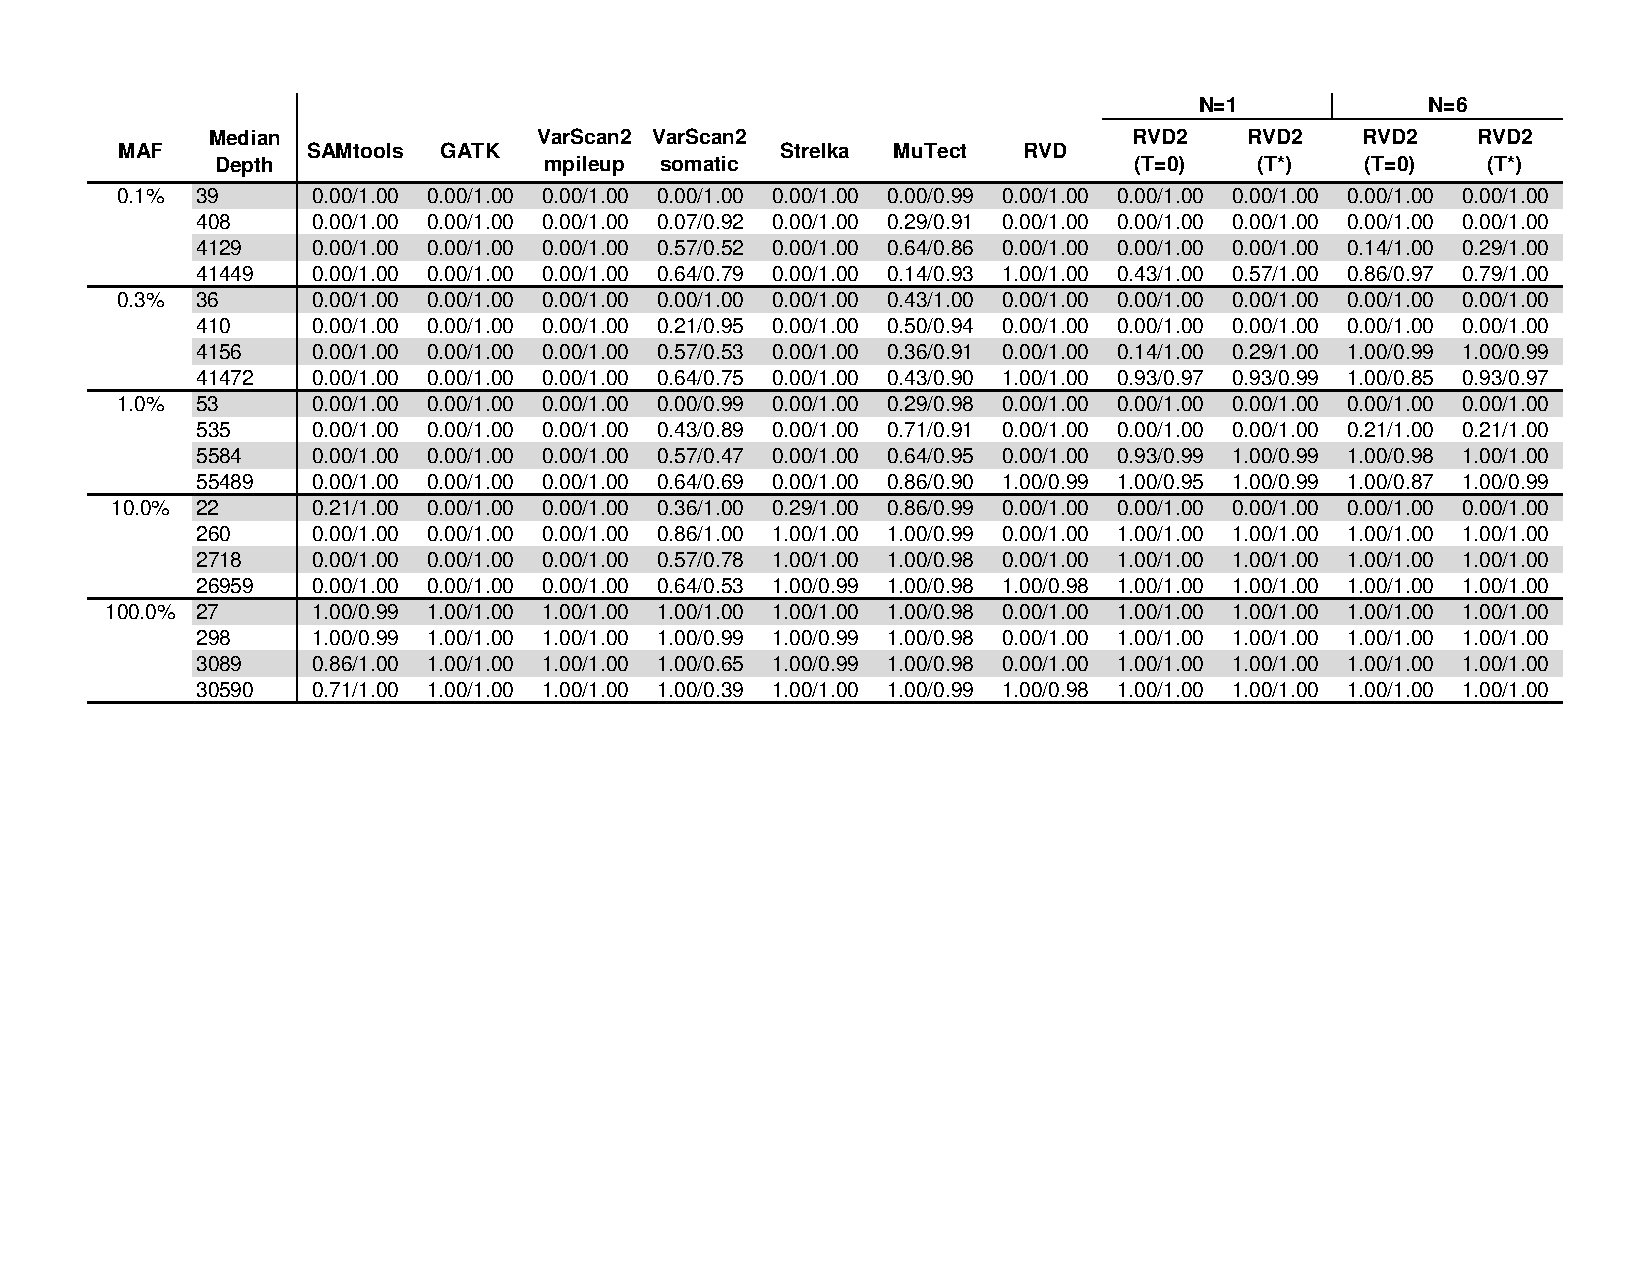
\includegraphics[width=0.84\textwidth]{pdf_figs/comparison_table_ss.pdf}
\caption{Sensitivity/Specificity comparison of RVD2 with other variant calling algorithms using synthetic DNA data.}
\vspace{-10pt}
\label{tbl:comparison_ss}
\end{figure*}

\begin{figure*}[!tbhp]
\centering
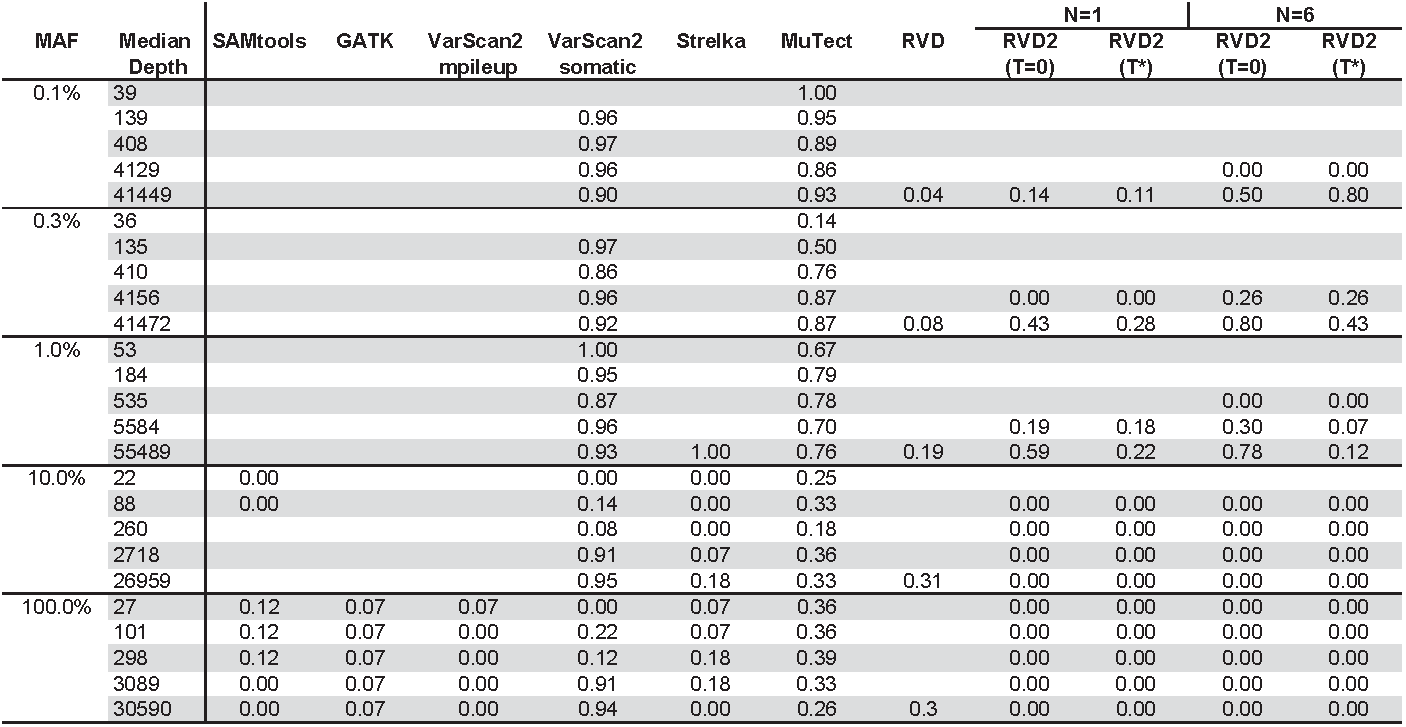
\includegraphics[width=0.84\textwidth]{pdf_figs/comparison_table_fdr.pdf}
\caption{False discovery rate comparison of RVD2 with other variant calling algorithms using synthetic DNA data. Blank cells indicate no locations were called variant.}
\vspace{-15pt}
\label{tbl:comparison_fdr}
\end{figure*}

Figure~\ref{tbl:comparison_ss} shows that samtools, GATK and VarScan2-mpileup all have similar performance. 
They call the 100\% MAF experiment well even at low depth, but are unable to identify true variants in mixed samples. 
VarScan2-somatic is able to call more mixed samples. However, as the read depth increases the specificity degrades. 
Strelka is able to call 10\% MAF variants with good performance, but is limited at 1\% MAF and below. 
muTect has good performance across a wide range of MAF levels. 
But even at the highest depth only has around 0.5 sensitivity for low MAF levels.

The performance statistics for RVD are an average of three sets of pair-end case replicates. 
RVD performed the best among all algorithms when the read depth is near 40,000. 
RVD called all the mutated positions across all MAF levels with no false positives when MAF level is 0.3\% or lower. 
However, RVD can not call any mutations when the depth is too low to measure the baseline error rate and therefore is not useful for low-depth data.

RVD2 has a high sensitivity and specificity for a broad range of read depths and minor-allele frequencies. 
The sensitivity increases considerably with read depth at a slight expense to specificity. 
For the most difficult test with a low read depth and low MAF, RVD2 performs on-par with muTect. 
With $\tau^*$ the performance is much better with high sensitivity and specificity across a wide range of read depths and MAFs. 
However, in practice one may not know the optimal $\tau^*$ a-priori. 
With $N=6$ replicates, the sensitivity increases considerably for low MAF variants with a slight degradation in specificity due to false positives. 
When the median read depth is at least $10\times$ the MAF, RVD2 has higher specificity than all of the other algorithms tested and has a lower sensitivity in only three cases.


\subsubsection*{False Discovery Rate Comparison}

Figure~\ref{tbl:comparison_fdr} shows the false discovery rate (FDR) for RVD2 compared to samtools, GATK, varscan, Strelka and muTect. 
Blank cells indicate no positive calls were made.

Samtools performs well on 100\% MAF sample and performance improves for read depths 3,089 and 30,590. 
GATK performs well on both the 10\% and 100\% variants, but makes a false positive call at the 100\% MAF level for all read depth levels. 
VarScan2-pileup performs perfectly for all but the lowest depth for the 100\% MAF.

VarScan2-somatic is able to make calls for all but the lowest MAF and coverage level. 
However, the FDR is high due to many false positives. Interestingly, at a MAF of 100\% the FDR is zero for lowest read depth and over 0.9 for the highest read depth. 
Strelka has a better FDR than the samtools, GATK or Varscan2-somatic algorithms for almost all read depths at the 10\% and 100\% MAF. 
However, it does not call any variants at or below 1\% MAF.  muTect has the best FDR performance of the other algorithms we tested over a wide range of MAF and depths. But the FDR level is relatively high at around 0.7 for 0.1\% -- 1\% MAF and 0.3 for 10\% -- 100\% MAF. 
RVD has best FDR performance in the high read depth for 0.1\% -- 1\% MAF levels. 
The FDR increases to around 0.3 for 10\% -- 100\% MAF in the high read depth.

RVD2 has a lower FDR than other algorithms when the read depth is greater than $10\times$ the inverse MAF with $N=1$ and $\tau$ set to the default value of zero or to the optimal value. 
The FDR is higher when $N=6$ because the variance of the control error rate distribution $P(\mu_j^{\text{control}} | r^{\text{control}})$ is smaller. The smaller variance yields improvements in sensitivity at the expense of more false positives. 
Since the FDR only considers positive calls, the performance by that measure degrades.

\vspace{-10pt}
\subsection{HCC1187 primary ductal carcinoma sample}\label{sec:brca}
\begin{figure*}[!hbpt]
\centering
\vspace{-10pt}
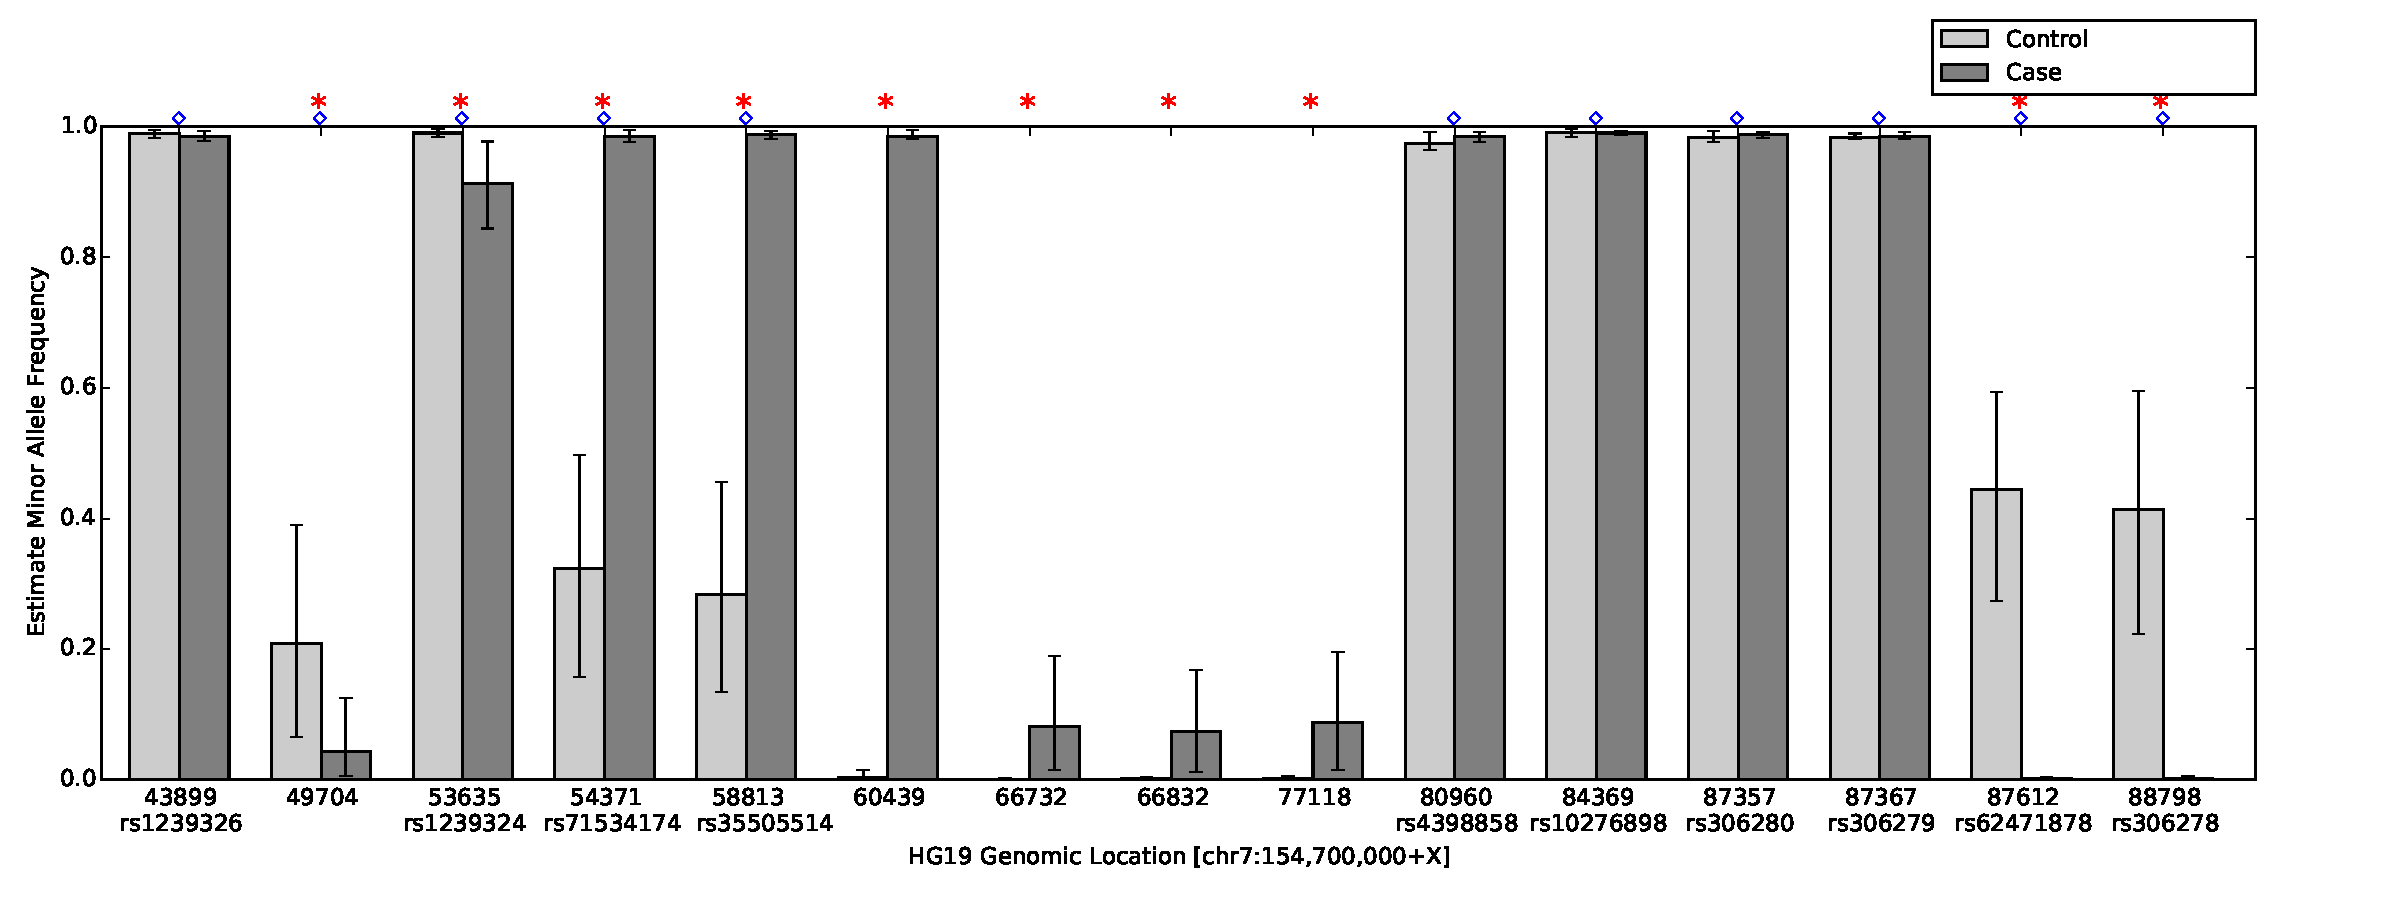
\includegraphics[width=0.9\textwidth]{pdf_figs/HCC1187_MuBarPlot.pdf}
\caption{Estimated minor allele fraction for germline and somatic mutations called by RVD2 in the 59kbp PAXIP1 gene. Blue diamonds ($\diamond$) indicates germline mutations, where $\mu^{\text{control}}$ is significantly different from the reference sequence. Red stars (*) indicates somatic mutations, where $\mu^{\text{case}}$ is significantly different from $ \mu^{\text{control}}$. The  vertical lines represent 95\% credible interval around posterior mean MAF. Ten positions are common population SNPs according to dbSNPv138, and the identities are shown below the positions.}
\vspace{-10pt}
\label{fig:brca_MAF}
\end{figure*}
% figure 5 generated from 2014-03-24_germline_and_somatic_test_correction_no_subclassification


\begin{figure*}[!pthb]
\vspace{-10pt}
    \centering
    \subfloat[\label{fig:brca_dot:a}]{{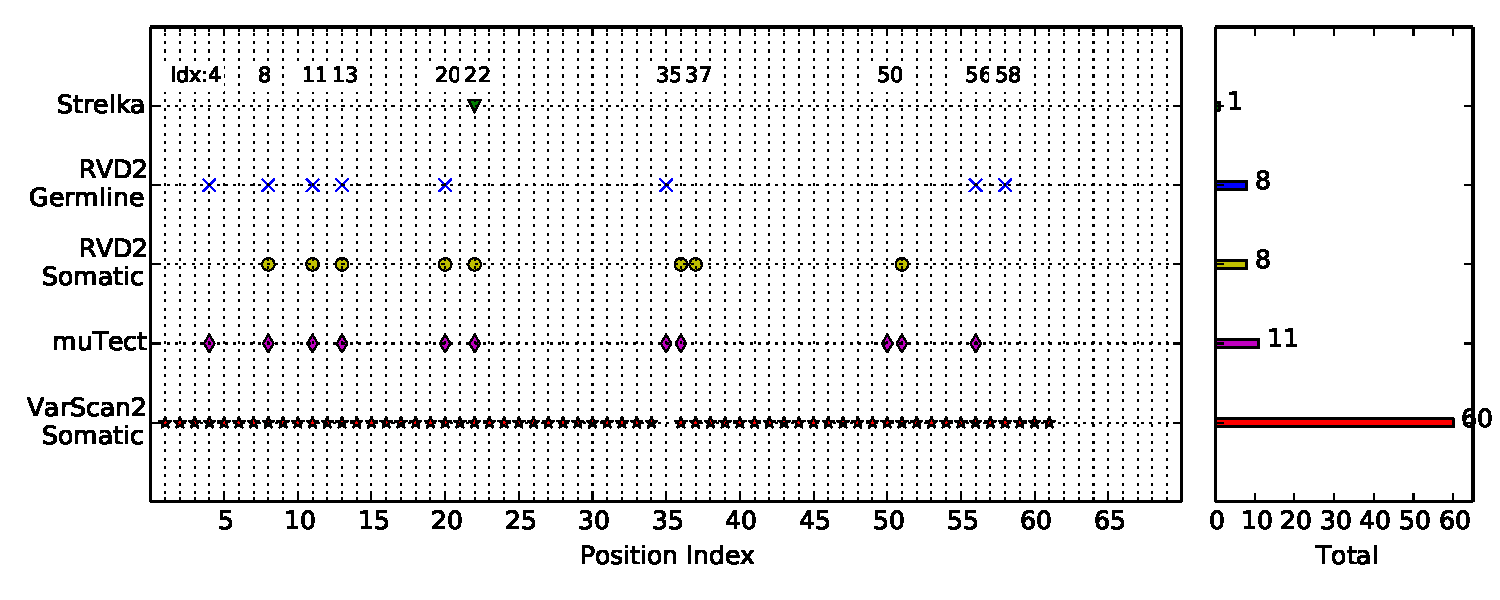
\includegraphics[width=0.8\textwidth]{pdf_figs/HCC1187_dotplot.pdf} }}%
    %
    \subfloat[\label{fig:brca_dot:b}]{{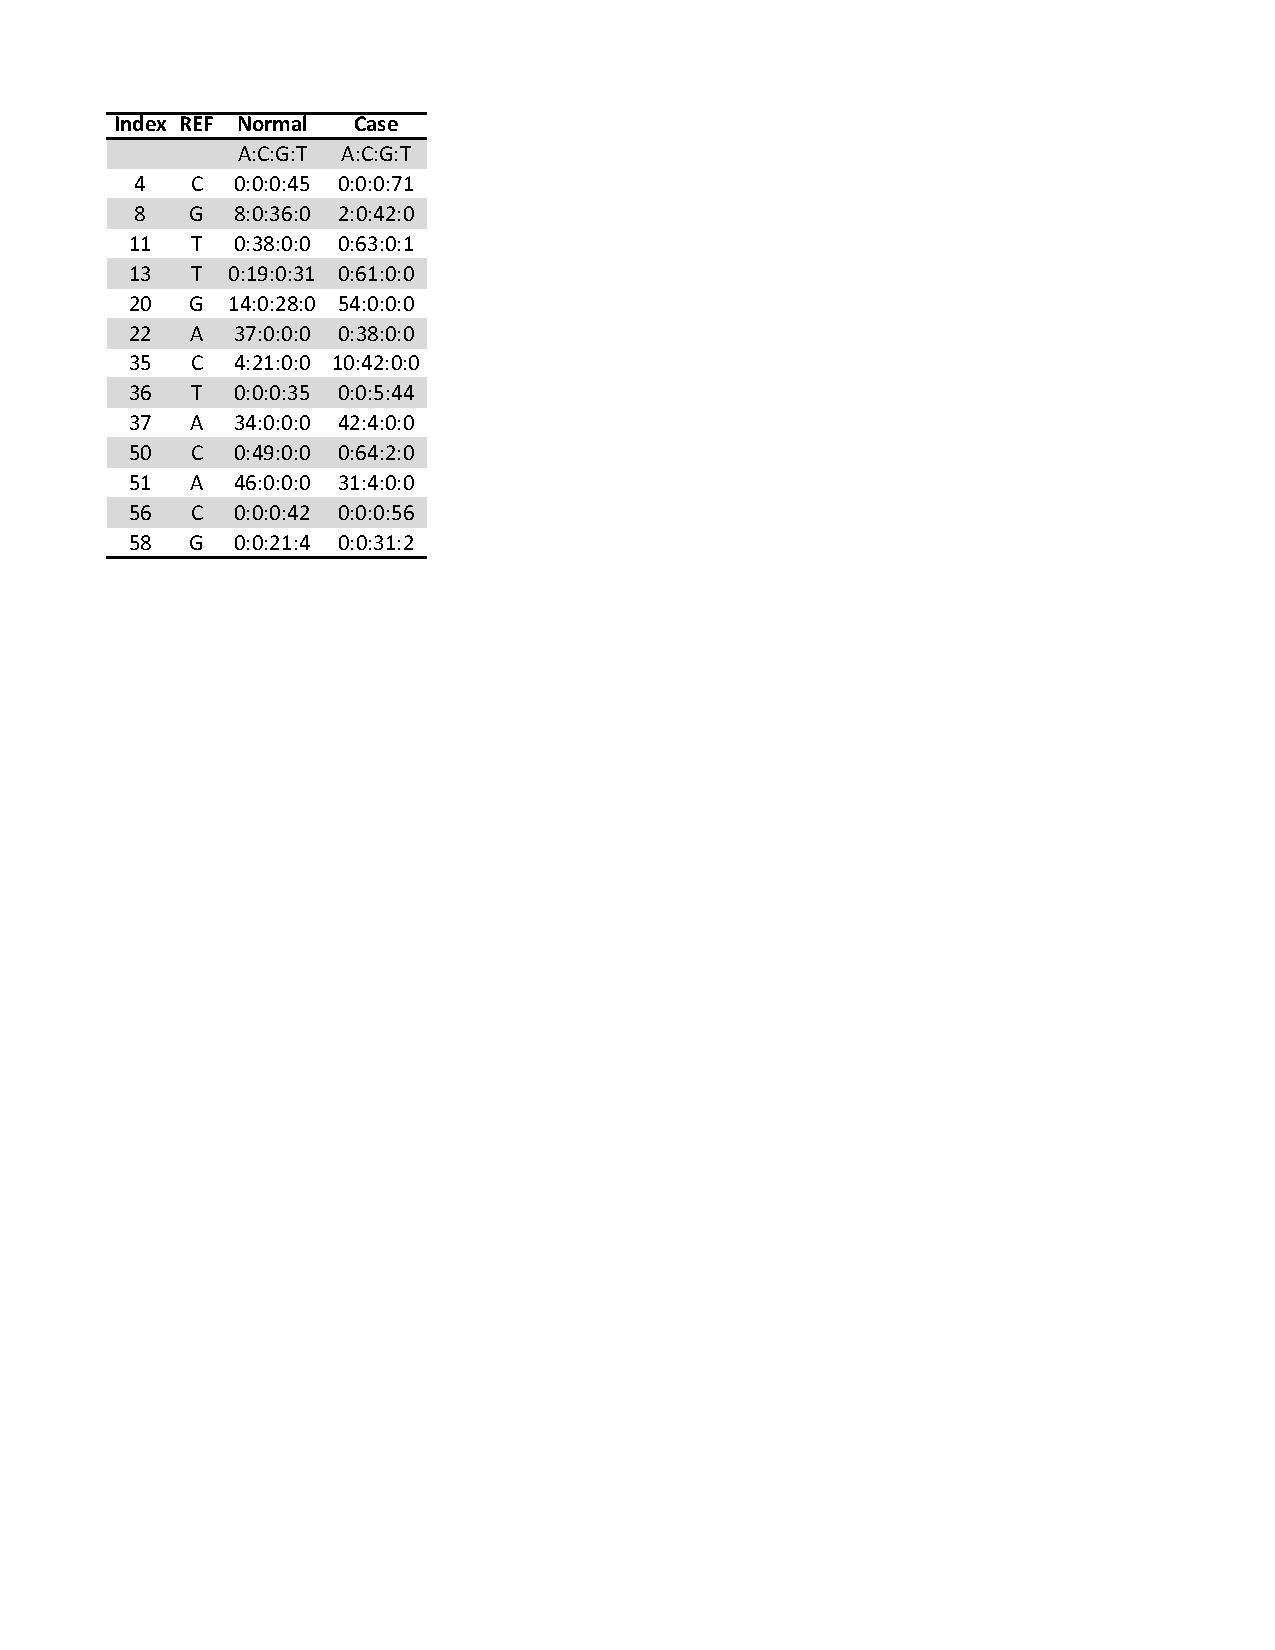
\includegraphics[width=0.21\textwidth]{pdf_figs/position_lookup_chart.pdf} }}%
    \caption{(a) Positions called by VarScan2-somatic, muTect, RVD2 and Strelka in the 59kbp PAXIP1 gene from chr7:154,735,400 to chr7:154,794,682. The positions are sorted by index (correspondance to genomic positions shown in Supplementary Table 1) (b) Read counts for each base for positions called by RVD2 and muTect from raw pileup data.}%
    \label{fig:brca_dot}%
\vspace{-10pt}
\end{figure*}

% figure 6 generated from 2014-03-12_dot_plot_mutation_detection_result_HCC1187_dataset

RVD2 identified twelve variants in the 59kbp PAXIP1 gene from chr7:154,735,400 to chr7:154,794,682. There were 11 germline variants and 10 somatic mutations. %Especially, two heterozygous germline variants had a loss-of-heterozygosity (LOH) in the tumor sample.
Figure~\ref{fig:brca_MAF} shows the estimated minor allele frequencies for the normal and tumor samples at the called locations. 
Positions 
chr7:154,743,899C\textgreater T, 
chr7:154,749,704G\textgreater A, 
chr7:154,753,635T\textgreater C, 
chr7:154,754,371T\textgreater C, 
chr7:154,758,813G\textgreater A, 
chr7:154,780,960C\textgreater T, 
chr7:154,784,369A\textgreater G, 
chr7:154,787,357C\textgreater T, 
chr7:154,787,367C\textgreater T, 
chr7:154,787,612A\textgreater G, and 
chr7:154,788,798A\textgreater G 
were called germline mutations. 
%
Positions 
chr7:154,749,704G\textgreater A, 
chr7:154,753,635T\textgreater C, 
chr7:154,754,371T\textgreater C, 
chr7:154,758,813G\textgreater A, 
chr7:154,760,439A\textgreater C, 
chr7:154,766,732T\textgreater G,  
chr7:154,766,832A\textgreater C,
chr7:154,777,118A\textgreater C,
chr7:154,787,612A\textgreater C,
chr7:154,788,798A\textgreater C, and
were identified as significantly different in tumor and normal sample and called somatic mutations.
% 
Positions chr7:154,754,371 and chr7:154,758,813 appear to be loss-of-heterozygosity events. 
Some of these mutations are also found to be common population SNPs according to dbSNPv138. 
The corresponding identities are shown in the Figure~\ref{fig:brca_MAF}. The read depth distribution for positions called by RVD2 are provided in Supplementary Table 1. 
%According to dbSNPv138 chr7:154743899 is rs1239326, chr7:154753635 is rs1239324, chr7:154754371 is rs71534174, chr7:154758813 is rs35505514, and chr7:154780960 is rs4398858.

\subsubsection{Performance comparison with other algorithms.}

We ran muTect and VarScan2-somatic to call mutations in the PAXIP1 gene in HCC1187 sample. We also compared to the result shown in original research report where Strelka was used to identify mutations in the same sample ~\citep{hcc1187techreport}. Figure~\ref{fig:brca_dot:a} shows mutation detection result from Strelka, RVD2, muTect, and VarScan2-somatic. For notation simplicity, we use position index to present actual positions in Figure~\ref{fig:brca_dot} (the corresponding genomic positions are provided in Supplementary Table 1). 

The mutations called by RVD2 and muTect are the most consistent among all the techniques. RVD2 detected twelve germline and somatic mutations, while muTect reported eleven; ten were called by both. In the disagreements, RVD2 did not call position 50 while muTect did not call position 37 and 58. Referring to the depth distribution shown in Figure~\ref{fig:brca_dot:b}, it can be seen that position 37 and 58 are more likely mutated while position 50 is less likely mutated. 

Strelka was the least sensitive algorithm among all the algorithms. According to the technical report, Strelka identified position 22 (chr7:154760439) as variant, but did not call any other variants. In particular Strelka missed the two LOH events called by RVD2. VarScan2-somatic called most positions among all algorithms, sixty positions as shown in Figure~\ref{fig:brca_dot:a}. VarScan2-somatic  detected all the positions called by RVD2 except position 35, which turns out to be a very likely mutation given the depth distribution in Figure~\ref{fig:brca_dot:b}. VarScan2-somatic reported fifty positions which were not called by any other three algorithms. The read depth in Supplementary Table 1 suggestions that these positions are very likely to be false positives. The fact that VarScan2-somatic can be over-sensitive has appeared in synthetic dataset analysis. As shown in Figure~\ref{tbl:comparison_fdr}, the false discovery rate for VarScan2-somatic at read depth 53 MAF level 1.0\% is as high as 1.00.  \citet{spencer2013performance} also mentioned that VarScan2 has tendency to call many false positives at high read depth. 
% To compare the performance of RVD2 with other algorithms, we used Strelka to identify mutationin the same sample. Strelka found three positions: chr7:154754371, chr7:154758813 and chr7:154760439.
\vspace{-5pt}
\section{Discussion}
We describe here a novel algorithm for model estimation and hypothesis testing for identifying single-nucleotide variants in heterogeneous samples using next-generation sequencing data. Our algorithm has a higher sensitivity and specificity than many other approaches for a range of read depths and minor allele frequencies.

Our inference algorithm uses Gibbs sampling to do inference in the RVD2 hierarchical empirical Bayes model. This sampling procedure provides a guarantee to identify the global optimal parameter settings asymptotically. However, it may require many samples to achieve that guarantee causing the algorithm to be slower than other deterministic approaches. We opted for this balance of speed and accuracy because computational time is often not limiting and the cost of a false positive or false negative greatly outweighs the cost of more computation. Another factor that can affect the speed of RVD2 is the number of Metropolis-Hasting sample within one Gibbs sampling run. RVD2 is able to use multiple cores in parallel, which can significantly improve time efficiency. On a computational node with 64 2.34GHz processor and 256Gb of RAM, RVD2 takes around 10 minutes to analyze the one 400bp long synthetic data set. The memory requirement is roughly the size of the gene sequence times the number of Gibbs samples. We are currently developing a variational method to estimate RVD2, aiming at decreasing computational time. 

We have focused on the statistical model and hypothesis test in this study and our results do not include any pre-filtration of erroneous reads or post-filtration of mutation calls beyond a simple quality score threshold. Incorporation of such data-cleaning steps will likely improve the accuracy of the algorithm.

Our approach does not address identification of indels, structural variants or copy number variants. Those mutations typically require specific data analysis models and tests that are different than those for single-nucleotide variants. Furthermore, analysis of RNA-seq data or other data generated on the NGS platform may require different models that are more appropriately tuned to the particular noise feature of that data.

The availability of clinical sequence data is increasing as the technical capability to sequence clinical samples at low cost improves. Consequently, we require statistically accurate algorithms that are able to call germline and somatic point mutations in heterogeneous samples with low purity. Such accurate algorithms are a step towards greater access to genomics for clinical diagnostics.

\vspace{-5pt}
\section*{Acknowledgements}
P.F. and Y.H. were supported by seed funding from Worcester Polytechnic Institute. Y.H. was supported by PhRMA Foundation Informatics Grant 2013080079.

\bibliographystyle{natbib}
\bibliography{bioinfo}
\end{document}
